\documentclass[12pt, a4paper]{article}

\title{Physics 2}
\date{} 

% This first part of the file is called the PREAMBLE. It includes
% customizations and command definitions. The preamble is everything
% between \documentclass and \begin{document}.
	
	\usepackage[margin=1in]{geometry}  % set the margins to 1in on all sides
	\usepackage{graphicx}              % to include figures
	\usepackage{amsmath}               % great math stuff
	\usepackage{amsfonts}              % for blackboard bold, etc
	\usepackage{amsthm}                % better theorem environments
	\usepackage{wrapfig}			   % for images formatting
	\usepackage{booktabs}
	\usepackage{caption}			   % for labeling images
	\usepackage{bigints}			   % for bigger integral symbols	
	\usepackage{subcaption}			   % subfigures functions
%	\usepackage{subfig}				   % subfigures
	
	% various theorems, numbered by section
	
	\newtheorem{thm}{Theorem}[section]
	\newtheorem{lem}[thm]{Lemma}
	\newtheorem{prop}[thm]{Proposition}
	\newtheorem{cor}[thm]{Corollary}
	\newtheorem{conj}[thm]{Conjecture}
	
	\DeclareMathOperator{\id}{id}
	
	\newcommand{\bd}[1]{\mathbf{#1}}  % for bolding symbols
	\newcommand{\RR}{\mathbb{R}}      % for Real numbers
	\newcommand{\ZZ}{\mathbb{Z}}      % for Integers
	\newcommand{\col}[1]{\left[\begin{matrix} #1 \end{matrix} \right]}
	\newcommand{\comb}[2]{\binom{#1^2 + #2^2}{#1+#2}}

	\begin{document}
	
		\section*{1. Coulomb's Law}
		
		\textbf{Coulomb's Law} describes the force between two charged particles. If the charges have the same sign, they repel, if they are opposite, they attract. The \textbf{electrostatic force} is given by:
		
		\begin{equation}
			\vec{F} = k \frac{q_1 q_2}{r^2} \hat{r} \tag{Coulomb's Law, 1-1}
		\end{equation}
		
		where:
		\begin{itemize}
			\item $\vec{F}$ is the force,
			\item $q_1$ and $q_2$ are the charges,
			\item $r$ is the distance between them,
			\item $k$ is a constant (\textbf{electrostatic constant}),
			\item $\hat{r}$ is a unit vector along the line connecting the charges.
		\end{itemize}
		
		Coulomb's Law is similar to \textbf{Newton's Law of Gravitation}, which gives the gravitational force between two masses as:
		
		\begin{equation}
			\vec{F} = G \frac{m_1 m_2}{r^2} \hat{r} \tag{Newton's Law of Gravitation, 1-2}
		\end{equation}
		
		Both laws follow an inverse-square relationship, meaning the force decreases with the square of the distance between the objects. However, unlike gravitational forces (which are always attractive), electrostatic forces can be either attractive or repulsive depending on the charges.
		
		Coulomb's law has been experimentally validated and works even at the atomic level, explaining the forces between atomic nuclei and electrons. It also accounts for the forces that bind atoms and molecules together.
		
		In the \textbf{SI unit system}, the unit of charge is the \textit{coulomb} (C), and \textbf{electric current} $i$ is defined as the rate at which charge flows:
		
		\begin{equation}
			i = \frac{dq}{dt} \tag{Electric Current, 1-3}
		\end{equation}
		where $i$ is the current (in ampères) and $dq$ is the charge (in coulombs) passing through a point in time $dt$.
		Rearranging in \textbf{SI} tells us that: 
		
		\begin{equation*}
			1C = (1A)(1s)
		\end{equation*}
		For historical reasons the constant $k$ is usually written as $1/4\pi\varepsilon_0$, therefore the magnitude in Coulomb's Law becomes
		
		\begin{equation}
			\textbf{F} = \frac{1}{4\pi\varepsilon_0} \frac{|q_1||q_2|}{r^2} \tag{Coulomb's Law, 1-4}
		\end{equation}
		The constants in Eqs. 1.1 and 1.4 have values:
		\begin{equation*}
			k = \frac{1}{4\pi\varepsilon_0} = 8.99 \cdot 10^9  \frac{N\cdot m^2}{C^2} 
		\end{equation*}
		The quantity $\varepsilon_0$ is called \textbf{permittivity constant of free space}:
		\begin{equation*}
			\varepsilon_0 = 8.85 \cdot 10^{-12} \frac{C^2}{N\cdot m^2}
		\end{equation*}
		Another parallel between the gravitational force and the electrostatic force is that they both obey the principle of superposition. Given $n$ charged particles we can say that the net force is given by the vector sum:
		\begin{equation*}
			\vec{F_{1,net}} = \vec{F_{1,2}} + \vec{F_{1,3}} + \vec{F_{1,4}} + ... + \vec{F_{1,n}} \tag{1-5}
		\end{equation*}
		
		\subsection*{1.1 Charge is Quantized}
		By experimental means we know that \textbf{charge} $q$ is \textbf{quantized}, thus any positive or negative charge that can be detected can be written as 
		\begin{equation*}
			q = n\cdot e,\quad\quad\quad n = \pm1, \pm2, \pm3,...
		\end{equation*}
		in which $e$, the \textbf{elementary charge}, has the approximate value: 
		\begin{equation*}
			e = 1.602 \cdot 10^{-19} C
		\end{equation*}
	
		
		\section*{2. The Electric Field}
		The \textbf{electric field} is a vector field that consists of a distribution of vectors around a charged object. We can define the electric field around a point $P$ by placing a certain charge $q_0$ at the point and then we measure the electrostatic force $\vec{F}$ that acts on the charge. We define the electric field $\vec{E}$ at a point $P$ due to a charged object as
		\begin{equation*}
			\vec{E} = \frac{\vec{F}}{q_0} \tag{Electric Field 2-1}
		\end{equation*}
		
		\textbf{Electric Field Lines} are graphical visual aid which consists of imaginary integral curves that are tangent to the \textbf{field vector} at any point along their length.
		
		\begin{figure}[ht]
			\centering
			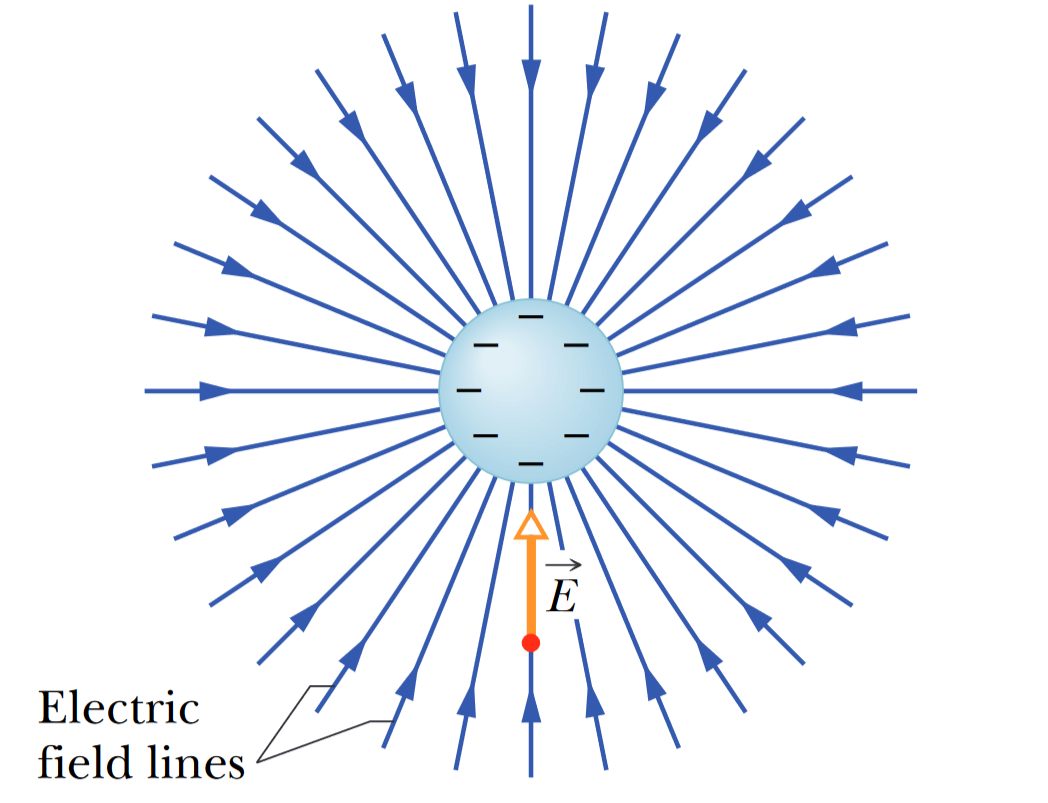
\includegraphics[width=8cm]{Physics2_PNGs/elec-field-lines.png}
			\caption{Electric Field Lines}
			\label{fig:electric-field-lines}
		\end{figure}
		
		
		\subsection*{2.1 Electric Fiels due to a Point Charge}
		To find an electric charge due to a point $q$ at any point to a distance $r$, we put a positive charge $q_0$. The \textbf{electrostatic force} acting on $q_0$ is:
		\begin{equation*}
			\vec{F} = \frac{1}{4\pi\varepsilon_0} \frac{q q_0}{r^2} \hat{r} 
		\end{equation*}
		The direction of $\vec{F}$ points directly away from the point charge is $q$ is positive, towards the point charge if $q$ is negative.
		The \textbf{electric field vector} is:
		\begin{equation*}
			\vec{E} = \frac{\vec{F}}{q_0} = \frac{1}{4\pi\varepsilon_0} \frac{q}{r^2} \tag{Point Charge, 2-2}
		\end{equation*}	
		$\vec{E}$ and $\vec{F}$ have same direction.
		
		We can quickly find the resultant electric field due to more than one point
		charge by placing a positive charge $q_0$ near $n$ point charges $q_1, q_2, . . . , q_n$, then,
		from Eq. 1-5, the net force from the n point charges acting on the test charge is:
		\begin{equation*}
			\vec{F_{0}} = \vec{F_{01}} + \vec{F_{02}} + \vec{F_{03}} + ... + \vec{F_{0n}}.
		\end{equation*}
		Therefore the net electric field at the position of the charge is:
		\begin{equation*}
			\vec{E} = \frac{\vec{F_0}}{q_0} = \frac{\vec{F_{01}}}{q_0} + \frac{\vec{F_{02}}}{q_0} + ... + \frac{\vec{F_{0n}}}{q_0} = \sum_{i=1}^{n} \frac{\vec{F_{0i}}}{q_0} = \sum_{i=1}^{n} \vec{E_i} \tag{2-3}
		\end{equation*}
	
		
		\subsection*{2.2 Electric Field due to an Electric Dipole}
		
		\begin{wrapfigure}{r}{0.25\textwidth}
			\centering
			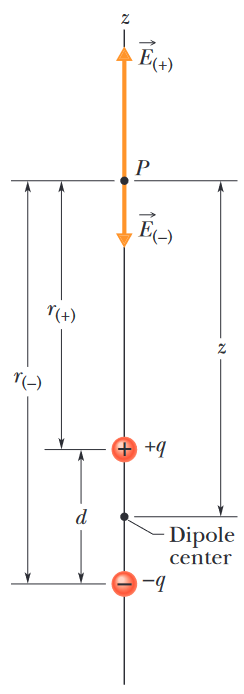
\includegraphics[width=3.5cm]{Physics2_PNGs/elec-dipole.png}
			\caption{An Electric Dipole}
			\label{fig:electric-dipole}
		\end{wrapfigure}
	
		An \textbf{Electric Dipole} consists of two charges of magnitude $q$, but opposite signs, separated by a distance $d$. The point of interest $P$ is located along the the \textbf{Dipole Axis} at a distance \textit{z} from the dipole's midpoint. 
		
		Due to the simmetry of this setup, the electric field components from the two charges ($E_{+}$ and $E_{-}$) must lie along the dipole axis which we have taken to be \textit{z} axis. Applying the \textbf{superposition principle} for electric fields, we find that the magnitude \textbf{E} at a point $P$ is: 
		\begin{equation*}
			\textbf{E} = E_{+} + E_{-}
		\end{equation*}
		\begin{equation*}
			= \frac{1}{4\pi \varepsilon_0} \frac{q}{r^2_{(+)}} - \frac{1}{4\pi \varepsilon_0} \frac{q}{r^2_{(-)}}
		\end{equation*}
		\begin{equation*}
			= \frac{q}{4\pi \varepsilon_0(\textit{z}-\frac{1}{2}d)^2} - \frac{q}{4\pi \varepsilon_0(\textit{z}+\frac{1}{2}d)^2}.
		\end{equation*}
		With a little algebra:
		\begin{equation*}
			\textbf{E} = \frac{q}{4\pi\epsilon_0\textit{z}^2}\biggl(\frac{1}{(1-\frac{d}{2\textit{z}})^2 } - 
			\frac{1}{(1+\frac{d}{2\textit{z}})^2 }\biggl).
		\end{equation*}
		\begin{equation*}
			\textbf{E} = 
			\frac{q}{4\pi \varepsilon_0\textit{z}^2} 
			\frac{2d/ \textit{z}}{\small(1-(\frac{d}{2\textit{z}})^2)^2}
			= \frac{q}{2\pi \varepsilon_0\textit{z}^3} 
			  \frac{d}{ (1 - (\frac{d}{2\textit{z}})^2)^2 }
			  \tag{2-4}
		\end{equation*}
	
		We are usually interested in the electrical effect of the dipole only at distances larger than the dipole, such distances as $\textit{z} \gg d$.
		At such distances, we have $d/2\textit{z} \ll 1$ in Eq. 2-4. Given this approximation, we can rewrite 2-4 as:
		\begin{equation*}
			\textbf{E} = \frac{1}{2\pi\varepsilon_0} \frac{qd}{\textit{z}^3}
			\tag{2-5}
		\end{equation*}
		
		The product $qd$ is the magnitude $\textbf{p}$ of a vector called  \textbf{Electric Dipole Moment} ($\vec{p} = q\vec{d}$). Thus we can rewrite 2-5 as:
		\begin{equation*}
			\textbf{E} = \frac{1}{2\pi\varepsilon_0} \frac{p}{\textit{z}^3}
			\tag{Electric Dipole, 2-6}
		\end{equation*}
		The direction of $\vec{p}$ is taken to be from the negative to the positive side of the dipole.
		
		
		\subsection*{2.3 Electric Field due to a Line of Charge}
		
		\begin{wraptable}{r}{0pt} 
			
			$ \begin{array}{crrr}
				 Name & Symbol & \text{SI Unit} \\
				\toprule
				Charge & q & C \\
				\text{Linear Charge Density} & \lambda & C/m \\
				\text{Surface Charge Density} & \sigma & C/m^2 \\
				\text{Volume Charge Density} & \rho & C/m^3 \\
				\bottomrule
			\end{array} $
			\caption{Some Measures of Electric Charge}
		\end{wraptable}
		
		We now consider \textbf{continuous} charge distributions. Given a ring of radius $R$ of uniform positive linear charge density $\lambda$ around its circumference, a differential element of charge occupies a length $ds$. This element sets up an electrical field $d\vec{E}$ at a point $P$. The component of $d\vec{E}$ along the central axis can be intercepted by $dE\cos\theta$.
		Therefore every element $ds$ has a charge of magnitude 
		\begin{equation*}
			dq = \lambda ds \tag{2-6}
		\end{equation*}
		This differential charge sets up a differential electric field $\vec{E}$ at a point $P$, which is at a distance $r$ from the point. Using Eq. 2-6 we can rewrite Eq. 2-2:
		\begin{equation*}
			dE = \frac{1}{4\pi\varepsilon_0} \frac{dq}{r^2} 
			   = \frac{1}{4\pi\varepsilon_0} \frac{\lambda ds}{r^2}
			   \tag{22-7}
		\end{equation*}
		
		\begin{wrapfigure}{r}{0.25\textwidth}
			\centering
			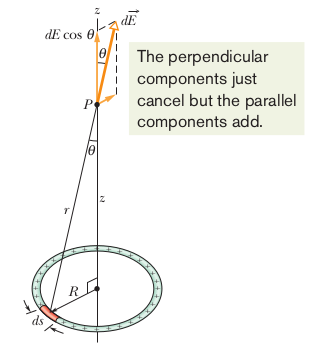
\includegraphics[width=6.07cm]{Physics2_PNGs/elec-line-charge.png}
			\caption{A Ring of Uniform Positive Charge}
			\label{fig:electric-line-of-charge}
		\end{wrapfigure}
		From Figure 3 we can rewrite Eq. 2-7: 
		\begin{equation*}
			dE = \frac{1}{4\pi\varepsilon_0} \frac{\lambda ds}{(\textit{z}^2 + R^2)}
				\tag{2-8}
		\end{equation*}
		Every $d\vec{E}$ has a component perpendicular to the central axis $\textit{z}$ ($d\vec{E}\cos\theta$) with equal magnitude but different direction. \\
		Therefore: 
		
		\begin{equation*}
			\begin{cases}
				\cos\theta = \scalebox{1.6}{$ \frac{\textit{z}}{r} $} = 
				\scalebox{1.4}{$ 
					\frac{\textit{z}}{(\textit{z}^2 + R^2)^{1/2}} $} \\ \\
				dE = \scalebox{1.3}{$\frac{1}{4\pi\varepsilon_0} \frac{\lambda ds}{(\textit{z}^2 + R^2)} $}
			\end{cases}\,.
		\end{equation*}
	
		Multiplying the first expression for the second gives us:
		\begin{equation*}
			d\vec{E}\cos\theta = \frac{\textit{z}\lambda}{4\pi\varepsilon_0(\textit{z}^2+R^2)^{3/2}}ds
			\tag{2-9}
		\end{equation*}
		
		To add the parallel components ($dE\cos\theta$) produced by all elements we integrate Eq. 2-9 around the circumference of the ring, from $s = 0$ to $s = 2\pi R$:
		\begin{equation*}
			E = \int dE\cos\theta = \frac{\textit{z}\lambda}{4\pi\varepsilon_0(\textit{z}^2+R^2)^{3/2}} \cdot
			\int_{0}^{2\pi R}ds = 
 			\frac{\textit{z}\lambda (2\pi R)}{4\pi\varepsilon_0(\textit{z}^2 + R^2)^{3/2}} 
			\tag{2-10}
		\end{equation*} 
		Since $\lambda$ is the charge per length of a ring, the term $\lambda2\pi R$ is just $q$ [$q = \lambda(2\pi R)$]:
		\begin{equation*}
			\scalebox{1.1}{$E$} = 
				\frac{\scalebox{1.2}{$q\textit{z}$}}
				     {\scalebox{1.3}{$4\pi\varepsilon_0(\textit{z}^2 + R^2)^{3/2}$}}
			\tag{Charged Ring, 2-11}
		\end{equation*}
		This equation yields the same results even if $q$ is negative. \\
		If we assume that $\textit{z} \gg R$, $\textit{z}^2 + R^2$ can be approximated as $\textit{z}^2$ and 2-11 becomes:
		\begin{equation*}
			E = \frac{q\textit{z}}{4\pi\varepsilon_0 \textit{z}^2} \tag{Charged Ring ad Large Distances, 2-12}
		\end{equation*}
		
		
		\subsection*{2.3.1 A Field Guide for Lines of Charge}
		Finding the electric field $\vec{E}$ produced at a point $P$ by a line of uniform charge, either circular or straight. The strategy is to pick on an element $dq$ of charge, find $d\vec{E}$ due to that element and integrate $d\vec{E}$ over the entire line of charge.
		\begin{itemize}
			\item[\textbf{Step 1.}] If the line of charge is circular, let $ds$ be the arc length of an element of the distribution. If the line is straight, sum on $x$ axis along it and let $dx$ be the length of an element.
			
			\item[\textbf{Step 2.}] Relate $dq$ of the element to the length of the element with either $dq = \lambda ds$ or $dq = \lambda dx$. Consider $dq$ and $\lambda$ positive even if the charge is actually negative.
			
			\item[\textbf{Step 3.}] Express the field $d\vec{E}$ produced at $P$ by $dq$ with
			$\vec{E} = \frac{\vec{F}}{q_0} = \frac{q}{4\pi\varepsilon_0r^2}$, replacing $q$ with either $q = \lambda ds$ or $q = \lambda dx$. If the charge on the line is positive then at $P$ draw a vector $d\vec{E}$ that points directly away from $dq$, opposite if the charge is negative.
			
			\item[\textbf{Step 4.}] Always look for any simmetry in the situation. If $P$ is on an axis of simmetry of the charge distribution, resolve the field $d\vec{E}$ produced by $dq$ into components that are perpendicular and parallel to the axis of simmetry. Repeat with the simmetric element $dq'$ and draw the vector $d\vec{E}'$ at $P$. One of the components produced by $dq$ is a cancelling component, cancelled by the corrisponding component produced by $dq'$, we have a similar concept in adding components. Integration is a way to add them up.
			
			\item[\textbf{Step 5.}] There are four general types of uniform charge distribution:
				\begin{itemize} 
					\item[Ring:] With point $P$ on the central axis of simmetry. In the expression for $d\vec{E}$ replace $r^2 = \textit{z}^2 + R^2$. Express the adding components of $d\vec{E}$ in terms of $\theta$. That introduces $\cos\theta$, but $\theta$ is identical to all the elements, therefore is not a variable. Replace $\cos\theta = \frac{\textit{z}}{r} = \frac{\textit{z}}{(\textit{z}^2 + R^2)^{1/2}}$ and integrate over $s$ around the circumference.
					
					\item[Circular Arc:] Point $P$ at the center of the curvature. Express the adding component of $d\vec{E}$ in terms of $\theta$. That introduces either $\sin\theta$ or $\cos\theta$. Reduce the two resulting variables $s$ and $\theta$ by replacing $ds = rd\theta$ from one end of the arc to the other.
					
					\item[Straight Line:] with point $P$ on an extension of the line (as in Fig. 4a). In the expression for $dE$, replace $r$ with $x$. Integrate over $x$ from end to end.	
					
					\item[Straight Line:] with point P at perpendicular distance $y$ from the line of charge  (Fig. 4b). In the expression for $dE$ replace $r$ with an expression involving $x$ and $y$. If $P$ is on the perpendicular bisector of the line of charge, find an expression for the adding component of $d\vec{E}$. That will introduce either $\sin\theta$ or $\cos\theta$. Reduce the resulting two variables $x$ and $\theta$ to one, $x$, by replacing the trigonometric function with an expression involving $x$ and $y$. Integrate over $x$ from end to end of the line of charge. If $P$ (Fig. 4c) is not on the line of simmetry, set up an integral to sum the components $dE_x$ and integrate over $x$ to find $E_x$. Also set up an integral to sum the components $dE_y$, integrate over $x$ again to find $E_y$. Now use $E_x$ and $E_y$ to find magnitude and direction of $\vec{E}$.
					
				\end{itemize}
			
			\item[\textbf{Step 6.}] One arrangement of the integration limits gives a positive result. The reverse gives the same result with a minus sign. Discard the minus sign. If the result is to be stated in terms of the total charge $Q$ of the distribution, replace $\lambda = Q / L$ in which $L$ is the length of the distribution.
			
		\end{itemize}
	
		\begin{figure}
			\centering
			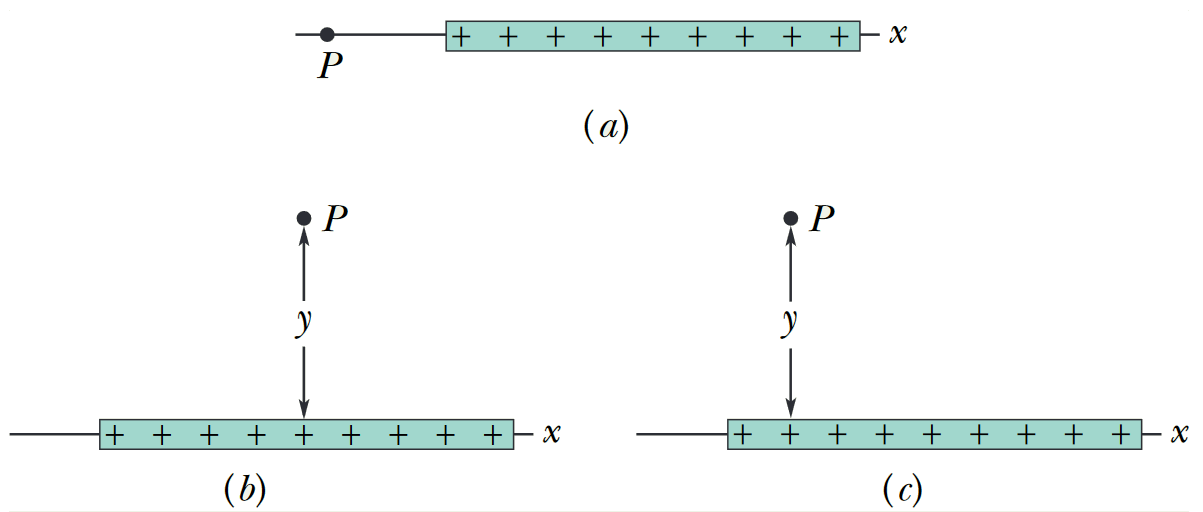
\includegraphics[width=10cm]{Physics2_PNGs/electric-line-charge.png}
			\caption*{Figure 4}
			\label{fig:line-of-charge}
		\end{figure}
	
	
		\subsection*{2.4 Point Charge in an Electric Field}
		
		\begin{wrapfigure}{r}{0.25\textwidth}
			\centering
			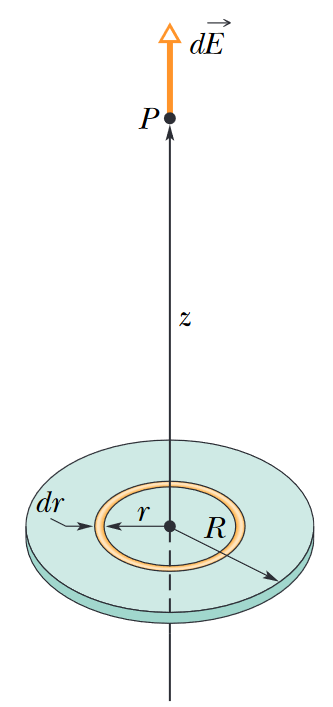
\includegraphics[width=3cm]{Physics2_PNGs/elec-charged-disk.png}
			\caption*{Figure 5: A disk of uniform positive charge}
			\label{fig:charged-disk}
		\end{wrapfigure}
	
		Figure 4 shows a circular plastic disk of $radius$ $R$ that has a positive surface charge of uniform density $\sigma$ on its upper surface. We need to find the electric field at point $P$, with distance $z$ from the disk along its central axis.
		We divide the disk into concentric flat rings and then calculate the electric field at point $P$ by adding up (integrating) the contribution of all rings. Fig. 4 shows one such ring, with radius $r$ and radial width $dr$. The charge on the ring is:
		
		\begin{equation*}
			dq = \sigma dA = \sigma (2\pi rdr)
			\tag{2-13}
		\end{equation*} 
		
		where $dA$ is the differential area of the ring. \\
		Substituting $dq$ from Eq. 2-13 for $q$ in Eq. 2-11:
		
		\begin{equation*}
			dE = \frac{z\sigma 2 \pi rdr}{4\pi\varepsilon_0(z^2 + r^2)^{3/2}}
		\end{equation*}
		which we can rewrite as
		\begin{equation*}
			dE = \frac{\sigma z}{4\varepsilon_0} \frac{2rdr}{(z^2 + r^2)^{3/2}}
			\tag{2-14}
		\end{equation*}
	
		We can now find $E$ by integrating 2-14 over the surface of the disk, with respect to the variable $r$ from $r = 0$ to $r = R$. We get
		\begin{equation*}
			E = \int dE = \frac{\sigma z}{4\varepsilon_0} \int_{0}^{R} (z^2 + r^2)^{-3/2}(2r)dr
			\tag{2-15}
		\end{equation*}
	
		This is easily solvable by casting the integral in the form $\int X^mdX$, by setting \\ $X = (z^2 + r^2),\quad dX = (2rdr)$  and  $ m = -\frac{3}{2}$, we have
		\begin{equation*}
			\int X^m dX = \frac{X^{m+1}}{m+1}
		\end{equation*}
	
		The solved integral becomes
		\begin{equation*}
			E = \frac{\sigma z}{4\varepsilon_0} \biggl[\frac{(z^2 + r^2)^{-1/2}}{-\frac{1}{2}} \biggl]_{0}^{R}
			\tag{2-16}
		\end{equation*}
	
		Taking the limits and rearranging we obtain:
		\begin{equation*}
			\textit{\textbf{E}} = \frac{\sigma}{2\varepsilon_0} \biggl(1 - \frac{z}{\sqrt{z^2 + R^2}} \biggl)
			\tag{Charged Disk, 2-17}
		\end{equation*}
		
		If we let $R \rightarrow \infty$ while keeping $z$ finite, the equation reduces to
		\begin{equation*}
			E = \frac{\sigma}{2\varepsilon_0}
			\tag{2-18}
		\end{equation*}
		This is the electric field produced by an infinite sheet of uniform charge. We get the same result by letting $z \rightarrow 0$ while keeping $R$ finite.
		
		
		
		\subsection*{2.5 Point Charge in an Electric Field}
		
		\begin{equation*}
			\vec{F} = q\vec{E}
			\tag{2-19}
		\end{equation*}
		
		The electrostatic force $\vec{F}$ acting on a charged particle located in an external electric field $\vec{E}$ has the direction of $\vec{E}$ if the charge $q$ of the particle is positive and has the opposite direction if $q$ is negative.
		
		
		\subsection*{2.6 A Dipole in an Electric Field}
		
		We have defined Dipole Moment ($\vec{p} =q\vec{d}$) as a vector that point from the negative to the positive end of the dipole. 
		A dipole in an Electric Field $\vec{E}$ consists of a rigid structure with two center of opposite charge and magnitude $q$. The dipole moment $\vec{p}$ makes an angle $\theta$ with $\vec{E}$. Electrostatic forces act on the charged ends of the dipole. Since $\vec{E}$ is uniform, those forces act in opposite directions with magnitude $F = qE$. Thus, since the field is uniform, the \textit{net force} on the dipole is $= 0$. However the forces on the charged ends produce a \textbf{net torque} $\vec{\tau}$ on the dipole in his center of mass, which lies in the line connecting the charged ends at some distance $x$ from one end and thus a distance $d - x$ from the other end. \\
		Given $\tau = rF\sin\phi$ we can write the magnitude of the net torque as:
		\begin{equation*}
			\tau = Fx\sin\theta + F(d-x)\sin\theta = Fd\sin\theta
			\tag{2-20}
		\end{equation*}
		or, by substituting $F = qE$ and $d = p / q$ we can find the magnitude of $\vec{\tau}$:
		\begin{equation*}
			\tau = pE\sin\theta
			\tag{2-21}
		\end{equation*}
		In a generalized vector form:
		\begin{equation*}
			\vec{\tau} = \vec{p} \times \vec{E}
			\tag{Torque on a Dipole, 2-22}
		\end{equation*}
	
		\begin{figure}
			\centering
			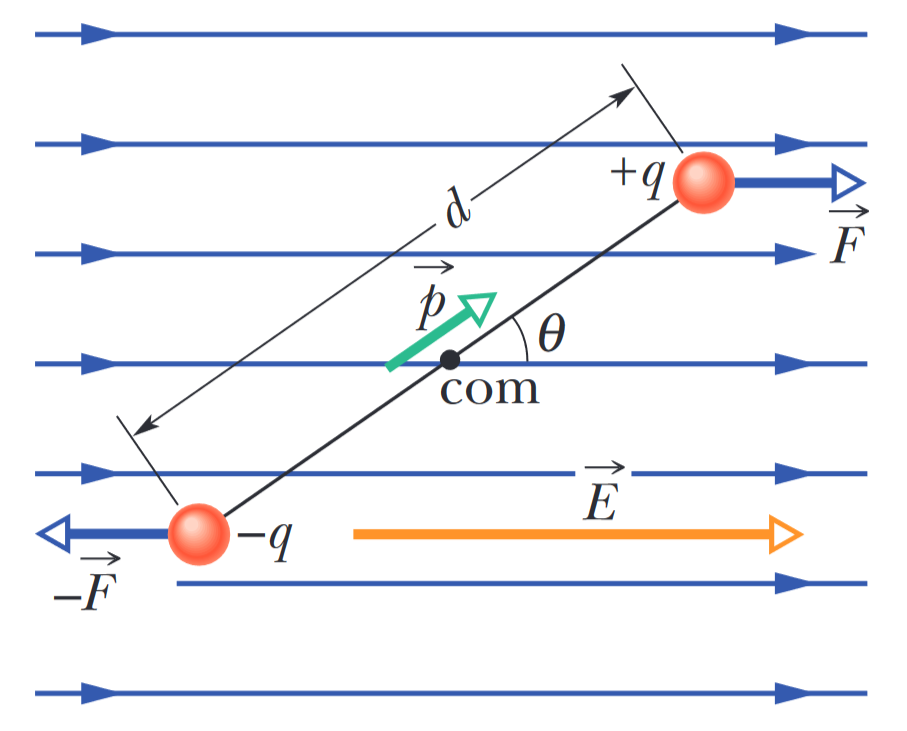
\includegraphics[width=5cm]{Physics2_PNGs/potential-dipole.png}
			\caption*{Figure 6: Dipole in an uniform external electric field $\vec{E}$}
			\label{fig:potential-dipole}
		\end{figure}
		
		
		\subsection*{2.7 Potential Energy of an Electric Dipole}
		
		We can associate potential energy with the orientaton of an electric dipole in an electric field. \\
		The dipole has less potential energy when it's in equilibrium orientation. Therefore when $\vec{\tau} = \vec{p} \times \vec{E} = 0$. The dipole is like a pendulum, which has the least gravitational potential energy in its equilibrium orientation. In any situation involvint potential energy we are free to define the 0 potential energy configuration. Given $\Delta U = -W$ and $W = \int \tau d\theta$ we find the potential energy at any angle $\theta$ to be:
		\begin{equation*}
			U = -W = -\int_{90^\circ}^{\theta} \tau d\theta = \int_{90^\circ}^{\theta} pE\sin\theta d\theta
			\tag{2-23}
		\end{equation*}
		Evaluating the integral leads to:
		\begin{equation*}
			U = -pE\cos\theta
			\tag{2-24}
		\end{equation*}
		We can generalize this equation in vectorial form as
		\begin{equation*}
			U = -\vec{p} \cdot \vec{E}
			\tag{Potential Energy of a Dipole, 2-25}
		\end{equation*}
		
		
		\newpage
		\section*{3. Gauss' Law}
		
		
		Gauss’ law relates the electric fields at points on a (closed) Gaussian surface to the net charge enclosed by that surface.
		
		
		\subsection*{3.1 Flux}
		
		Let's suppose a wide airstream of uniform velocity $\vec{v}$ at a small square loop of area $A$. Let \textbf{$\Phi$} represent the \textit{volume flow rate} at which the air flows thorugh the loop and let $\theta$ be the angle between the velocity $\vec{v}$ and the area vector $\vec{A}$ (a vector whose magnitude is equal to $A$ and whose direction is normal to the plane of the area $A$). We can now say that:
		\begin{equation*}
			\textbf{$\Phi$} = (v\cos\theta)A = \vec{v} \cdot \vec{A}
			\tag{3-1}
		\end{equation*}
		
		\begin{figure}[!htb]  % force figure under subsection
			\centering
			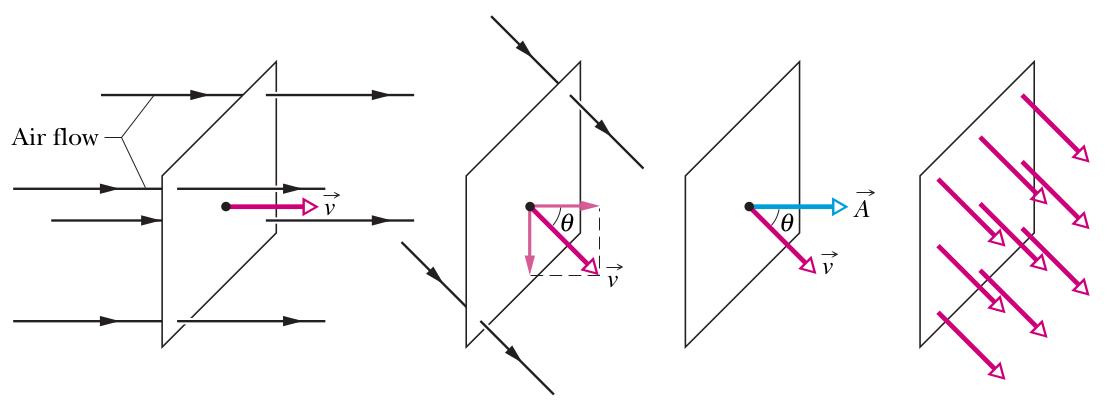
\includegraphics[width=10cm,height=3.5cm]{Physics2_PNGs/elec-veloc-flux.png}
			\caption*{Figure 7: An airstream $\vec{v}$ going through a square of area $A$}
			\label{fig:flux-over-square}
		\end{figure}
	
	
		\subsection*{3.2 Flux of an Electric Field}
		
		\begin{wrapfigure}{r}{0.15\textwidth}
			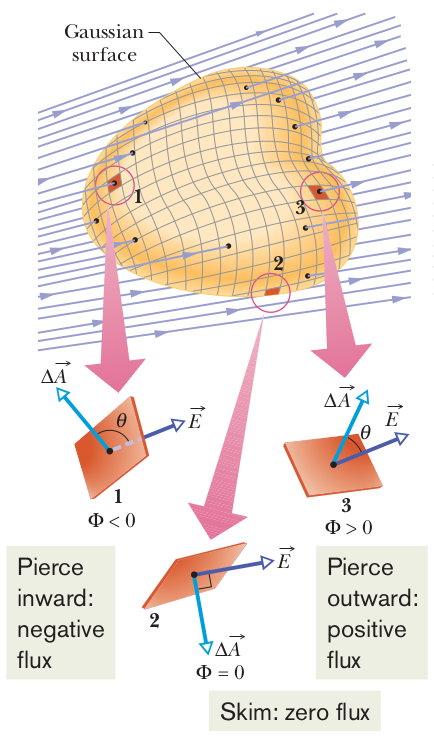
\includegraphics[width=4.5cm,height=7cm]{Physics2_PNGs/gaussian-elec-field.png}
			
			\label{fig:gaussian-elec-field}
		\end{wrapfigure}
		
		To define the flux of an electric field, we can take an arbitrary (asymmetric) Gaussian Surface immersed in a nonuniform electric field. Let us divide the surface into small squares of area $\Delta A$, small enough to neglect the curvature of the surface. We represent each of such element with an area vector $\Delta\vec{A}$.
		Given the small dimension of each square, we can treat the electric field $\vec{E}$ as constant over any given square. The vector $\Delta\vec{A}$ and $\vec{E}$ for each square make some angle $\theta$ with each other. A first definition for the flux of the electric field for a Gaussian Surface can be:
		\begin{equation*}
			\Phi = \sum \vec{E} \cdot \Delta\vec{A}
			\tag{3-2}
		\end{equation*}
		If we allow the area of each square to become smaller and smaller, we can approach a differential limit $dA$. The area vectors will therefore approach a differential limit $d\vec{A}$. \\ \\The sum 3-2 becomes a closed surface integral:
		\begin{equation*}
			\scalebox{1.3}{$ \mathbf{\Phi} = \bigointsss \vec{E} \cdot d\vec{A}$ }
			\tag{Electric Flux through a Gaussian Surface, 3-3}
		\end{equation*}
		The Flux of an Electric Field is a \textit{scalar}, and its \textbf{SI} unit is the \textit{newton-square-meter per coulomb} [$N \cdot m^2/C$] 
		
		\newpage
		\subsection*{3.2.1 Flux through a Closed Cylinder, Uniform Field}
		
		Given a \textbf{Cylinder}-shaped Gaussian Surface, with radius $R$ immersed in an \textbf{uniform} electric field $\vec{E}$, with the cylider axis parallel to the field. What is the flux $\mathbf{\Phi}$ of the electric field through this closed surface? \\
		We can find the flux $\mathbf{\Phi}$ by \textbf{integrating} the scalar product $\vec{E} \cdot d\vec{A}$ over the surface.
		We can do the integration by writing the flux as the sum of three terms: left cylinder cap $a$, the cylindrical surface $b$, right cylinder cap $c$. Thus:
		\begin{gather*}	% equation with newline
			\Phi = \bigointssss \vec{E} \cdot d\vec{A} 
			= \bigintssss_{a} \vec{E} \cdot d\vec{A}
			+ \bigintssss_{b} \vec{E} \cdot d\vec{A}
			+ \bigintssss_{c} \vec{E} \cdot d\vec{A} 	\tag{3-4} \\
				\bigintssss_{a} \vec{E} \cdot d\vec{A} 
					= \bigintssss_{a} E(\cos180^\circ) dA = E \cdot A = -\pi R^2 E	\\
				\bigintssss_{b} \vec{E} \cdot d\vec{A}  
					= \bigintssss_{b} E(\cos90^\circ) dA = 0	\\
				\bigintssss_{c} \vec{E} \cdot d\vec{A} 
					= \bigintssss_{a} E(\cos0^\circ) dA = E \cdot A = \pi R^2 E	\\
			\text	{Substituting into 3-4 yields:}  \\
			\Phi = -\pi R^2 E + 0 + \pi R^2 E = 0 \tag{Answer}
		\end{gather*}
		
		\begin{figure}[!htb]  % force figure under subsection
			\centering
			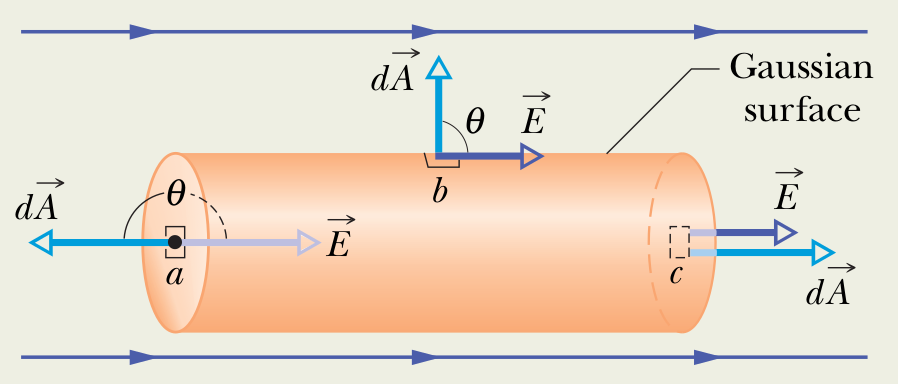
\includegraphics[width=8cm]{Physics2_PNGs/closed-cylinder.png}
			\caption*{}
			\label{fig:closed-cylinder}
		\end{figure}
		The net flux is zero because the field lines that represent the electric field all pass entirely through the Gaussian surface, from the left to the right.
		
		
		\subsection*{3.3 Gauss' Law}
		
		Gauss' Law relates the net flux $\Phi$ of an electric field through a closed surface (a Gaussian Surface) to the net charge $q_{enc}$ that is \textit{enclosed} by that surface. It tells us that:
		\begin{equation*}
			\varepsilon_0 \Phi = q_{\text{int}}
			\tag{Gauss' Law, 3-5}
		\end{equation*}
		By substituting 3-5 into the definition of Flux, we can also write Gauss' Law as:
		\begin{equation*}
			\varepsilon_0 \bigointssss \vec{E} \cdot d\vec{A} = q_{\text{int}}
			\tag{Gauss' Law, 3-6} 
		\end{equation*}
		These equations holds when the net charge is located in the void or in the air. The net charge $q_{enc}$ is the algebraic sum of all \textit{enclosed} positive and negative charges. \\ 
		If $q_{\text{int}} > 0$ the net flux is \textit{outward}; \\
		if $q_{\text{int}} < 0$ the net flus is \textit{inward}. \\
		Charges \text{outside} the surface are not included in the term $q_{\text{int}}$ in Gauss' Law. The exact form and location of the charges of the Gaussian Surface are also irrelevant. The only thing that matters on the right side of the equations are the magnitude and sign of the net enclosed charge. \\
		However the quantity $\vec{E}$ on the left side of Eq. 3-6 is the electric field resulting from all charges, both those inside and those outside the Gaussian Surface, this is due to the fact that the electric field due to a charge outside the Gaussian surface contributes zero net flux through the surface, because as many field lines due to that charge enter the surface as leave it. \\
		
		\begin{wrapfigure}{r}{0.17\textwidth}
			\centering
			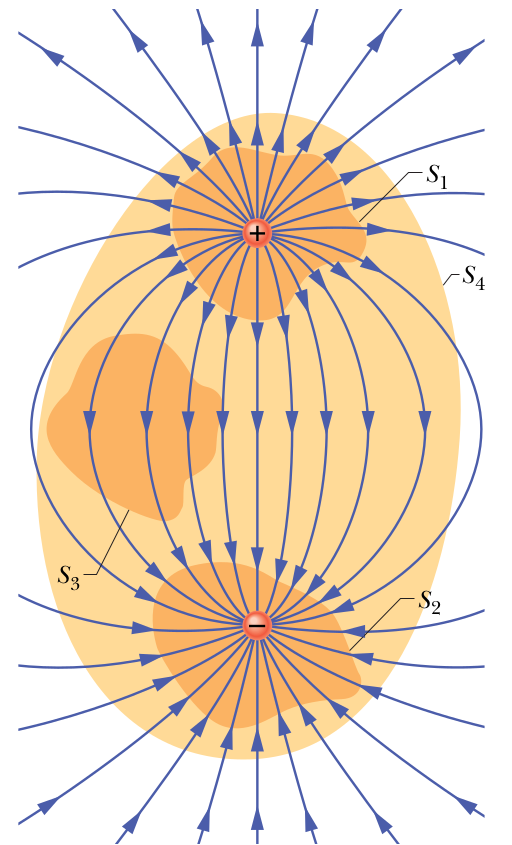
\includegraphics[width=4cm]{Physics2_PNGs/gaussian-surf-lines.png}
			\caption*{Figure 8}
			\label{gaussian-surf-lines}
		\end{wrapfigure}
		
		In Fig. 8 we have an example of two charges of \textbf{equal magnitude}, but \textbf{opposite sign}. Four Gaussian Surfaces are shown in cross section:
		\begin{itemize}
			\item[Surface $S_1$]: $\vec{E}$ is outward for all points, thus flux $\Phi > 0$ and $q_{\text{int}} > 0$.
			\item[Surface $S_2$]: $\vec{E}$ is inward for all points, thus flux $\Phi < 0$ and $q_{\text{int}} < 0$.
			\item[Surface $S_3$]: This surface encloses no charge, thus $q_{\text{int}} = 0$, by Gauss' Law also requires that net flux $\Phi = 0$.
			\item[Surface $S_4$]: This surface encloses no \textit{net} charge, because the enclosed positive and negative charges have equal magnitudes \\ 
			($q_{\text{int}} = q_1 - q_2 = 0$). Gauss' Law requires that net flux $\Phi = 0$.
		\end{itemize}
		\ \\ \\ 		
		
		\subsection*{3.4 Gauss' Law and Coulomb's Law}
		
		Since Coulomb's Law and Gauss' Law are different ways of describing the relationship between \textbf{electric charge} and \textbf{electric field} in static situations, we should be able to derive each from the other. \\
		Taken a positive point charge $q$ around which we drawn a concentric Gaussian surface of radius $r$. We can divide the surface into differential areas $dA$. By definition the area vector $d\vec{A}$ is perpendicular and pointed outwards at any point of the surface. From the simmetry of the situation, we know that the field $\vec{E}$ is also perpendicular to the surface and directed outward. Thus, since the angle $\theta$ between $\vec{E}$ and $d\vec{A}$ is zero, we can rewrite Eq. 3-6 for Gauss' Law as: 
		
		\begin{equation*}
			\varepsilon_0 \oint \vec{E} \cdot d\vec{A} =
			\varepsilon_0 \oint EdA = q_{\text{int}}
			\tag{3-7}
		\end{equation*}

		Here, $q_{\text{int}} = q$. Although $E$ varies radially with distance from $q$, it has same value everywhere on the spherical surface. We can draw the conclusion that E is constant, therefore:
		
		\begin{equation*}
			\varepsilon_0 E \oint dA = q.
		\end{equation*}
	
		The integral now is just the sum of all the points on the surface of the sphere, we can then rewrite the differential $dA$ over the surface of the sphere as ($4\pi r^2)$:
		
		\begin{equation*}
			\varepsilon_0 E (4\pi r^2) = q
		\end{equation*}
	
		or, rearranging:
		
		\begin{equation*}
			E = \frac{1}{4\pi\varepsilon_0} \frac{q}{r^2}
			\tag{3-8}
		\end{equation*}
		We can observe that the resulting equation is coherent with Coulomb's Law.


		
		\subsection*{3.5 A Charged Isolated Conductor}

		If an excess charge is placed on an isolated conductor, that amount of charge will move entirely to the surface of the conductor, thus none of the excess charge will be found within the body of the conductor ( Given by the fact that charges with same sign repel one another ).\\
		We take a Gaussian Surface just under the Conductor's Surface \\
		\begin{equation*}
			E = 0 \rightarrow \Phi = 0 \rightarrow q_{int} = 0 
		\end{equation*}
		The excess charge over an Isolated Conductor lays completely over the external surface.  \\\\
		The same principle applies to an Isolated Conductor with a cavity, its surface has no \text{excess} charge.
		
		
		\subsection*{3.6 External Electric Field}
		
		
		\begin{wrapfigure}{r}{0.17\textwidth}
			\centering
			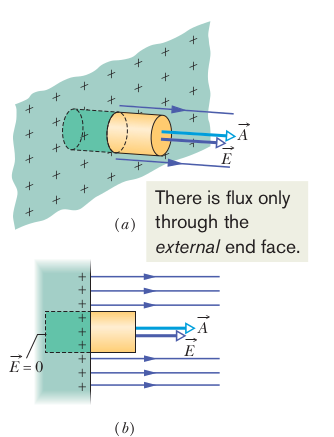
\includegraphics[width=5cm]{Physics2_PNGs/external-elec-field.png}
			\caption*{}
			\label{fig:external-elec-field.png}
		\end{wrapfigure}
		
		Overall, the charge does not distribute evenly over the Surface of a Conductor. 
	
		Eventhough there's a direct relationship between the field $\vec{E}$ and the (surface) Charge Density $\sigma$ $[ C/m^2 ]$.\\
		We take a small cylinder that encapsulates an element of the Surface. The field $\vec{E}$ is \textbf{perpendicular} to the surface (the charge would move otherwise). Therefore the charge $q_{\text{int}}$ enclosed by the Gaussian surface lies on the conductor's surface in an area $A$. Knowing that $\sigma$ is the charge per unit area, then $q_{\text{int}}$ is equal to $\sigma A$. Substituting $\sigma A$ for $q_{int}$ and $EA$ for $\Phi$, Gauss' law becomes:
		\begin{equation*}
			\varepsilon_0 EA = \sigma A 
			\tag{3-9}
		\end{equation*}
		from which we find:
		\begin{equation*}
			E = \frac{\sigma}{\varepsilon_0}
			\tag{Conducting Surface, 3-10}
		\end{equation*}
	
		\newpage
	
	
	
		\subsection*{3.7 Gauss' Law: Cylindrical Symmetry}
		
		Infinitely long cylindrical plastic rod with uniform positive linear charge density $\lambda$ $[ C/m ]$. Let's find an expression for the magnitude of the Electric field $\vec{E}$ at a distance $r$ from the axis of the rod. The Gaussian Surface we choose should match the simmetry of the problem (which is cylindrical).
		
		We choose a circular cylinder of radius $r$ and length $h$, coaxial with the rod. Any rotation of the rod (about its longitudinal axis) wouldn't make any change in the electric field. Therefore at every point on the cylindrical part of the Gaussian surface $\vec{E}$ must have the same magnitude $E$ and must directed radially outside (for a positively charged rod). \\
		
		Since $2\pi r$ is the cylinder circumference and $h$ is its height, the area A of the cylindrical surface is $2\pi rh$. The flux $\vec{E}$ through the surface is then
		\begin{equation*}
			\Phi = EA\cos\theta = E(2\pi rh)\cos0 = E(2\pi rh)
		\end{equation*}
		There is no flux through the end caps of the surface since $\vec{E}$ is radially directed, thus parallel to the end caps at every point.
		
		The charge enclosed by the surface is $\lambda h$, therefore
		\begin{equation*}
			\varepsilon_0 \Phi = q_{\text{int}}
		\end{equation*}
		reduces to
		\begin{equation*}
			\varepsilon_0 E(2\pi rh) = \lambda h
		\end{equation*}
	
		We can then describe the field around an infinitely long, straight rod of charge as
		\begin{equation*}
			E = \frac{\lambda}{2\pi\epsilon_0 r}
			\tag{line of charge, 3-11}
		\end{equation*}
	
		
	
	
		\subsection*{3.8 Gauss' Law: Planar Symmetry}
		
		\begin{wrapfigure}{r}{0.17\textwidth}
			\centering
			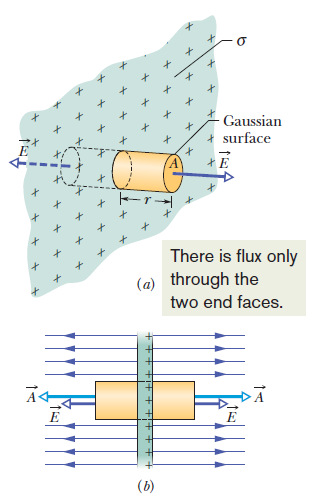
\includegraphics[width=4cm]{Physics2_PNGs/planar-gauss-surf.png}
			\caption*{}
			\label{fig:planar-gauss-surf.png}
		\end{wrapfigure}
		
		
		Thin, infinite, non-conducing sheet with an uniform (positive) surface charge density $\sigma$ $[ C/m^2 ]$. A useful Gaussian surface is a closed cylinder with end caps of area $A$, arranged to pierce the sheet perpendicularly as shown. From symmetry, $\vec{E}$ must be perpendicular to the sheet and hence to the end caps. Furthermore, since the charge is positive, $\vec{E}$ is directed \textit{away} from the sheet, and thus the electric field lines pierce the two Gaussian end caps in an outward direction. Because the field lines do not pierce the curved surface, there is no flux through this portion of the Gaussian surface. Thus, $\vec{E} \cdot d\vec{A}$ is simply $E \, dA$; then Gauss’ law,
		
		\begin{equation*}
			\varepsilon_0 \oint \vec{E} \cdot d\vec{A} = q_{\text{int}}
		\end{equation*}
		
		becomes
		
		\begin{equation*}
			\varepsilon_0 (EA + EA) = \sigma A,
		\end{equation*}
		
		where $\sigma A$ is the charge enclosed by the Gaussian surface. This gives
		
		\begin{equation*}
			E = \frac{\sigma}{2\varepsilon_0} \quad \text{(sheet of charge).}
			\tag{3-12}
		\end{equation*}
		
		Since we are considering an infinite sheet with uniform charge density, this result holds for any point at a finite distance from the sheet. Equation (3-12) agrees with Eq. 2-18, which we found by integration of electric field components.
		
		
		
		\subsection*{3.8.1 Two Conducting Plates}
		
		If there is no external electric field to force the positive charge into some particular distribution, it will spread out on the two faces with a uniform surface charge density of magnitude $\sigma$. From Eq. 3-10 we know that just outside the plate this charge sets up an electric field of magnitude
		
		\begin{equation*}
			E = \frac{\sigma}{\varepsilon_0}
		\end{equation*}
		Since the excess charge is positive, the field is directed away from the plate.
		
		\begin{wrapfigure}{r}{0.17\textwidth}
			\centering
			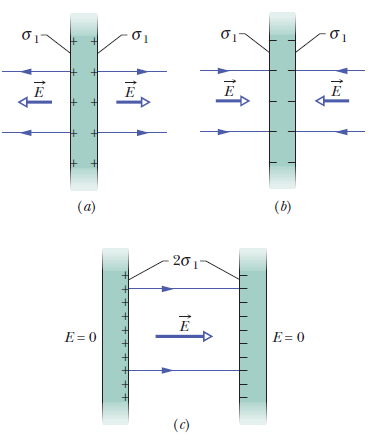
\includegraphics[width=5cm]{Physics2_PNGs/two-conducting-plates.png}
			\caption*{}
			\label{fig:two-conducting-plates.png}
		\end{wrapfigure}
		
		Figure 23-16b shows an identical plate with excess negative charge having the same magnitude of surface charge density $\sigma$. The only difference is that now the electric field is directed toward the plate.
		
		Suppose we arrange for the plates of a and b to be close to each other and parallel. Since the plates are conductors, when we bring them into this arrangement, the excess charge on one plate attracts the excess charge on the other plate, and all the excess charge moves onto the inner faces of the plates as in c. With twice as much charge now on each inner face, the new surface charge density (call it $\sigma_1$) on each inner face is twice $\sigma$. Thus, the electric field at any point between the plates has the magnitude
		
		\begin{equation}
			E = \frac{2\sigma_1}{\varepsilon_0} = \frac{\sigma}{\varepsilon_0}
			\quad \text{(two conducting plates)} \tag{3-13}
		\end{equation}
		
		This field is directed away from the positively charged plate and toward the negatively charged plate. Since no excess charge is left on the outer faces, the electric field to the left and right of the plates is zero.
		


		\subsection*{3.9 Gauss' Law: Spherical Symmetry}
		
		\begin{itemize}
			\item[1.] A shell of uniform charge attracts or repels a charged particle that is outside the shell
			as if all the shell’s charge were concentrated at the center of the shell.  
			\item[2.] If a charged particle is located inside a shell of uniform charge, there is no electrostatic
			force on the particle from the shell.
		\end{itemize}

		We have a charged spherical shell of total charge $q$ and radius $R$, and two concentric spherical Gaussian surfaces ( $S_1$ and $S_2$ ). Applying Gauss’ law to $S_2$ (for which $r \geq R$):
		
		\begin{equation}
			E = \frac{1}{4\pi\varepsilon_0} \frac{q}{r^2}, 
			\tag{(spherical shell, field at $r \geq R$), 3-14}
		\end{equation}
		This field is the same as the one set up by a point charge at the center of the shell. Apllying Gauss' law to $S_1$ (for which $r < R$):
		\begin{equation}
			E = 0,
			\tag{spherical shell, field at $r < R$, 3-15}
		\end{equation}
		Since the surface $S_1$ encloses no charge.
		
		Every distribution with spherical symmetry is a superposition of concentric layers. To apply the two shell theorems, each shell needs to have the same volume charge density $\rho$. Thus for the charge distribution as a whole $\rho$ can only vary with $r$. \\
		Letting $q'$ represent the charge enclosed by any  Gaussian surface, we can
		rewrite Eq. 3-14 as:
		
		\begin{equation}
			E = \frac{1}{4\pi\varepsilon_0} \frac{q'}{r^2},
			\tag{(spherical distribution, field at $r \leq R$), 3-16}
		\end{equation} 
		If the full charge $q$ is uniformly distributed, then $q'$ enclosed within radius $r$ is proportional to $q$:
		
		\[
		\frac{q'}{q} = \frac{\text{volume of sphere } r}{\text{volume of sphere } R}
		\quad \text{or} \quad
		\frac{q'}{\frac{4}{3} \pi r^3} = \frac{q}{\frac{4}{3} \pi R^3} 
		\tag{3-17}
		\]
		This gives us
		\[
		q' = q \frac{r^3}{R^3}
		\tag{3-18}
		\]
		Substituting this into Eq. 3-16 yields:
		\begin{equation*}
			E = \biggl( \frac{q}{4\pi\varepsilon_0 R^3} \biggl) r
			\tag{(uniform charge, field at $r \leq R$), 3-19}
		\end{equation*}
		
		\begin{figure}[h]
			\centering
			\begin{subfigure}{0.45\textwidth} % Adjust width as needed
				\centering
				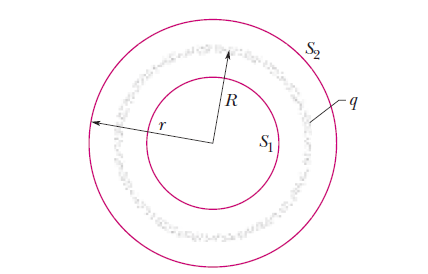
\includegraphics[width=6cm]{Physics2_PNGs/shell-theorem.png} % Replace with actual file
				\caption*{A thin, uniformly charged,
					spherical shell with total charge q, in cross
					section. Two Gaussian surfaces $S_1$ and $S_2$
					are also shown in cross section. Surface $S_2$
					encloses the shell, and $S_1$ encloses only the
					empty interior of the shell.}
				\label{fig:shell-theorem.png}
			\end{subfigure}
			\hfill
			\begin{subfigure}{0.45\textwidth} % Adjust width as needed
				\centering
				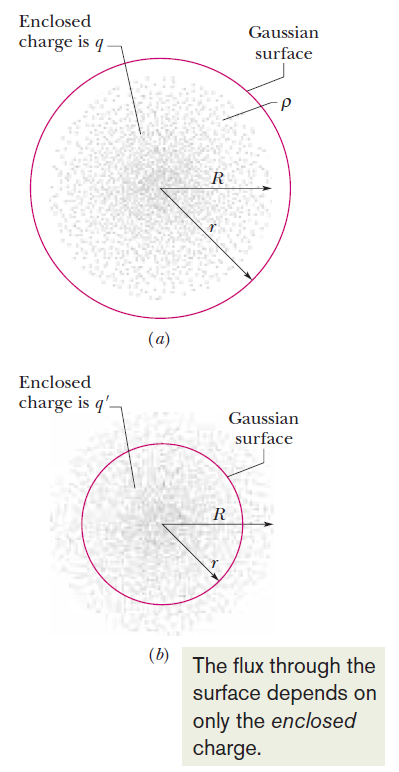
\includegraphics[width=4cm]{Physics2_PNGs/gauss-spherical-symm.png} 
				\caption*{}
				\label{fig:gauss-spherical-symm.png}
			\end{subfigure}
			\caption*{}
			\label{fig:both}
		\end{figure}
		\newpage
		
		
		
		
		\section*{4. Electric Potential}
		
		When an electrostatic force acts between two or more charged particles within a sistem, we can assign an \textbf{electric potential energy} $U$ to the system. If the system changes configuration from an initial state $i$ to a final state $f$, the electrostatic force does work $W$ on the system. We know that the resulting change $\Delta U$ in potential energy is:
	
		\begin{equation*}
			\Delta U = U_f - U_i = -W
			\tag{4-1}
		\end{equation*}
		The potential energy of a charged particle in an electric field varies according to the charge magnitude. However, the potential energy per unit charge [U/q] at any point in the electric field has a singular, definite value and it is called \textbf{electric potential} $V$ at that point (it is also a scalar, not a vector). Thus:
		\begin{equation*}
			V = \frac{U}{q}
			\tag{4-2}
		\end{equation*}
		We can then rewrite the \textit{electric potential difference} $\Delta V$ between two points $i$ and $f$ as:
		\begin{equation*}
			\Delta V = V_f - V_i = \frac{U_f}{q} - \frac{U_i}{q} = \frac{\Delta U}{q}
			\tag{4-3}
		\end{equation*}
		and by substituting $\Delta U =  -W$ we can define the \textit{potential difference} between poin $i$ and $f$ as:
		\begin{equation*}
			\Delta V = V_f - V_i = - \frac{W}{q}
			\tag{potential difference, 4-4}
		\end{equation*}
		By setting $U_f = 0$ at infinity as our reference potential energy, then the potential $V$ must be also 0. Therefore
		\begin{equation*}
			V = - \frac{W_{\infty}}{q}
		\end{equation*}
		The SI unit for potential is joule per coulomb [1 volt = 1 joule / coulomb] and allows us to assign a more conventional unit for electric field $\vec{E}$. By conversion we obtain
		\[
			1 \, N/C = \biggl( 1 \, \frac{N}{C} \biggl) \,
					   \biggl( \frac{1 \, V \cdot C}{1 \, J}\biggl) \,
					   \biggl( \frac{1 \, J}{1 \, N \cdot m} \biggl)
					 = 1 \, V / m
			\tag{4-5}
		\]
		We can also now define another useful unit in the atomic domain: one Electron-Volt (eV) is the energy equal to the work required to move a single elementary charge $e$ through a potential difference of one volt (1 $V$).
		\[
			1 \, \text{eV} = e(1 \text{V}) =  ( 1.60 \cdot 10^{-19} \text{C} )
			( 1 \, \text{J} / \text{C} ) = 1.60 \cdot 10^{-19} \text{J}
		\]
		We supposedly move a particle of charge $q$ from $i$ to $f$ in an electric field by applying a force to it, this force does work $W_{\text{app}}$ while the electric field does work $W$. By the work-kinetic energy theorem the change in kinetic energy $\Delta K$ of the particle is:
		\begin{equation*}
			\Delta K = K_f - K_i = W_{\text{app}} + W
			\tag{4-6}
		\end{equation*}
		We now suppose the particle is stationary before and after the move. Then $K_f$ and $K_i$ are both zero. Eq.4-6 reduces to
		\begin{equation*}
			W_{\text{app}} = -W
			\tag{4-7}
		\end{equation*}


	\end{document}